\chapter{Project Execution}
\label{chap:execution}

A topic-specific chapter, of roughly $15$ pages
This chapter is intended to describe what you did: the goal is to explain the main activity or activities, of any type, which constituted your work during the project.

The content is highly topic-specific, but for many projects it will make sense to split the chapter into two sections:
 - one will discuss the design of something (e.g., some hardware or software, or an algorithm, or experiment), including any rationale or decisions made,
 - and the other will discuss how this design was realised via some form of implementation.

This is, of course, far from ideal for {\em many} project topics.  Some
situations which clearly require a different approach include:
\begin{itemize}
\item In a project where asymptotic analysis of some algorithm is the goal,
      there is no real ``design and implementation'' in a traditional sense
      even though the activity of analysis is clearly within the remit of
      this chapter.
\item In a project where analysis of some results is as major, or a more
      major goal than the implementation that produced them, it might be
      sensible to merge this chapter with the next one: the main activity
      is such that discussion of the results cannot be viewed separately.
\end{itemize}


Note that it is common to include evidence of ``best practice'' project management (e.g., use of version control, choice of programming language and so on).
Rather than simply a rote list, make sure any such content is useful and/or informative in some way: for example, if there was a decision to be made then explain the trade-offs and implications involved.



\section{Introduction}
The main activity of this project was the development of a mobile app that can usefully analyse climbers' technique and then provide them with various data whilst they trainig or climb for fun.

\subsection{User-Centered Iterative Design}
aims

iteration

spiral

testing

\section{Initial Survey}
To inform my first forays into the project, I released a questionnaire online.
The questions can be found in Appendix~\ref{appx:survey} and my Ethics Application can be found in Appendix~\ref{appx:1-ea}.
I shared links to this survey across a variety of local climbing club pages, and received 49 responses in total. 
It must be mentioned that approximately half of these responses came in after I had already started development of the app, so although they did not all contribute to my initial development, I regularly checked the survey results and took into account any new opinions that were presented.
This is a benefit of an online survey, as I got a much broader reach, quantity and range of responses compared to if I had performed a more traditional paper survey at a climbing wall.

\clearpage
\subsection{Survey Respondents}
\begin{wrapfigure}{r}{8cm}
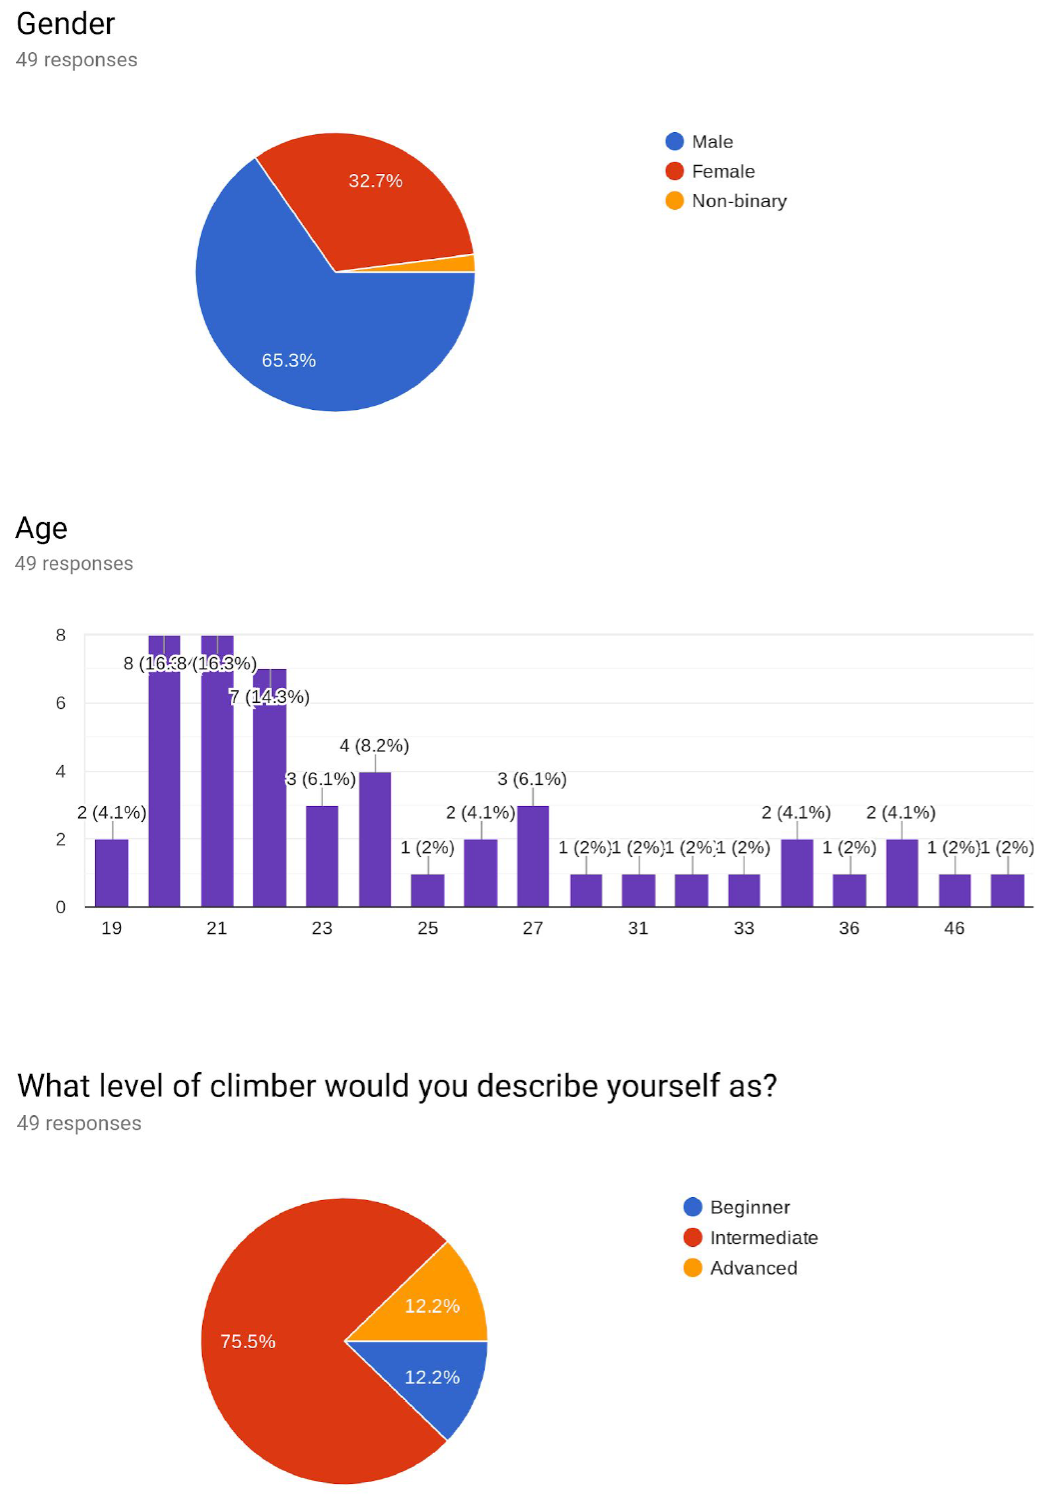
\includegraphics[width=7cm]{imgs/surveydemographics}
\caption{Demographics of Respondents to the Initial Survey}
\label{fig:surveydemographics}
\end{wrapfigure}
Some statistics on the demographics of the respondents can be seen in Figure~\ref{fig:surveydemographics}.

The male-female gender split is fairly consistent with the general indoor climbing population: 65\% male respondents compared to the 64\% stated in Rapelje's study on the demographics of climbers~\cite{climbing-sub-worlds}, and 65\% aged 19-24, compared to 60\% in that study.
This was aided by efforts to spread the survey link across a range of local climbing pages and Facebook Groups, not just the student groups to get a more representative sample of views.

With three-quarters of the respondents self-describing as intermediate climbers, the survey predominately hit the target audience for the project. 
Although all the responses were taken into account, a more heavy weighting was placed on the suggestions given by intermediates compared to the lower and higher abilities.



\subsection{Insights Gained From the Survey}
\subsubsection{Equipment Used}
To inform my decisions on what form my interactive device should take, I asked what items of equipment climbers often bring to the wall.
Everyone stated that they bring their own shoes, 90\% stated they bring a chalk-bag (a small hip-bag that contains powdered chalk for drying fingers and improving grip), and 31\% said they bring a small brush for cleaning dirty holds.

This provides a range of locations for locating a potential device, either inside the pocket of the chalk-bags, or attached to a brush, keeping with the light-weight aims of the project.

Only one respondent in this question included a phone in their list of equipment brought to the wall, and one even explicitly stated that they deliberately left their phone in their bag in order to "get away" from it. 
However, in later questions, an app (and thus a phone) was the most discussed potential device for usage, with multiple suggestions that a "you would severely limit your possible audience by having the need for a device" as "everyone has a phone" so I should "stick with an app".



\subsubsection{Communication With Others Whilst Climbing}
Because an potential use of the device was to aid some of the common interactions that climbers had with friends at the wall, two of the questions in this initial survey asked what kind of things people wanted to hear whilst climbing, and what they often told their friends.

The most common response was "beta", which is a colloqial climbing term for advice on how body-positioning should be used to solve a tricky climb. 
<insert a definition?>
This can vary a lot between climbers, with each climb usually having two or more potential solutions.
Also, being able to "read" a climb to determine this beta is a tough and much-sought-after skill within the climbing community, to the extent that it is often nearly impossible for the very best in the sport, and thus definitely out of reach of any artificial Intelligence I could hope to create within this project.
An alternative, which was suggested by a few survey respondents, could have been to record (with either video or other sensors) a proficient climber climbing that route, and then showing that at a later date. 
However, this data-collection and -replay contradicted my initial aim of the device/app being able to be used anywhere; I wouldn't want to have to go around every few months and re-record somebody climbing every climb at each climbing wall just for the product to remain usable.

Another common interaction highlighted by the survey was "pointing out holds" to a climber, who is often so engrossed in the climb that they do not notice a certain location that they could put their hands or feet.
This has an obvious potential use-case for a device, by using a colour video and existing computer-vision algorithms for coloured-blob-detection to find and then audio-relay the location of nearby holds to a climber, so this was selected to be examined further.



\subsubsection{Requested Potential Features}
Arguably the most useful question was the one asking
\textit{"Are there any features you'd like to see in a training app or device?"}.
This elicited a very wide range of suggestions, from yoga and meal plans to VR-viewing of someone climbing alongside.
Many of these were either too simple (and could be achieved by googling), or far too ambitious in scope.

The most common request was a way to log climbs in some way, and although a few logging apps already exist, this feature was definitely required in some way alongside whichever novel features were to be developed.
Tracking progression and seeing gradual improvements over time is a typical characteristic of training in any sport, but instead of simply listing climbs that had been done, a few respondents suggested that other metrics could be tracked, such as height climbed, frequent muscle groups used, and weak-points in technique that caused a climber to fall off at a certain point.


Many respondents emphasised that ease-of use was very important, so they didn't waste time climbing by clicking through the app.
"Large buttons for chalky fingers" were requested, alongside "a minimum of two clicks between opening the app and using it".

The video-analysis of technique was mentioned by seven respondents, with a mixture of technique-tutoring, centre-of-gravity detection and limb-annotation suggested.
Both centre-of-gravity and limb-annotation could be feasible achieved with computer-vision, so those were taken forward to the wizard-of-oz testing phase.
However, if beta-detection has been ruled out as too difficult for CV/AI, then giving accurate technique advice is even further out of the range of potential features: with the high complexity of movements in the sport, years of learning required to achieve coaching qualifications, and the high risk of injury if incorrect, giving explicit advice about how to climb is not something that I wanted to go into with this project.

One metric that was proposed is the analysis of efficiency or smoothness in a climb.
A commonly accepted signifier of "good technique" is when a climber moves neatly and directly between each successive climb, without any jerky motions or unnecessary readjustments.
A simple accelerometer recording could be used to determine this metric and thus this suggestion was also brought forward to the next stage of testing.



\section{Fundamental Early Decisions for Development}

\subsection{Platform Choice}
Despite researching a variety of different devices and form factors, one of the key aims of the project was always to make the final product as accessible as possible, therefore a OS-independent mobile app was decided upon after reviewing the survey results.
By not using any extra equipment such as wristbands or 3d-cameras, the scope and ability of the final product could be limited - eg by lack of sensors and processing power - however limiting the need for anything but just a phone, which almost everyone owns, was a worthwhile sacrifice.
As well as making user-testing much easier, this choice also helped narrow the down the direction of the project, as working solely within the limits of what a mobile app could achieve meant that the capabilities of that platform could be fully stretched and explored.

The two inputs that mobiles can easily capture and that would potentially be most useful for the analysis of climbing technique were video recordings and accelerometer data.
Video recordings can be analysed with various computer vision techniques, and accelerometer data can be shown on a graph and analysed statistically for various outputs.


\subsection{Tool Selection}
\subsubsection{Development tool}
Next was to find a app-development tool that is quick and easy to use (for quick repeated iterations of the app), can easily import or link to the OpenCV Library (for the computer vision aspect), and is platform-independant (so any mobile phone owners can use the app, irrespective of OS).

Unity was chosen as it meets all three of those requirements, with a wide variety of Assets that can be imported.
Also having used the tool for games development in the past I was very familiar with using Unity, and knew that iterating over app designs would be quick and easy enough, compared to potentially wasting time learning how to use other tools when this one met all the requirements with the added benefit of previous experience using the tool.

\subsubsection{Version Control}
For version-control I used \verb|git|, backed-up on GitHub.
Being a one-person project I rarely bothered with the overhead of using different branches, but the ability to roll-back to working code and releases, and to \verb|stash| and \stash|pop| various files at different times was very useful during development.
Once or twice a week, after a new feature or big set of fixes had been added, I would up-version the app, and release a compiled .apk binary to the project's GitHub page.
This allowed the easy re-installing of older versions when trying to locating a bug, as well as a clear documentation of all fixes and features included at each minor version upgrade.


\section{Initial Wizard-Of-Oz Study}
The initial survey showed interest in using computer vision to either give feedback about climbing technique, or to point out where nearby handholds were.
To those ends, I began experimenting with using OpenCV to detect blobs in previous recordings of my own climbing.

Although some small success was had in detecting the center of body mass, and some nearby coloured handholds, the wide variety of different lighting conditions and noise from the low-res camera made the detections very innaccurate.
Another issue that came up was that the code would analyse the video very slowly, even on my PC with a graphics card, so converting that to battery-efficient code that could run in real-time on a mobile device would have been extremely difficult.

Due to the time-scope of this project, and the aims being to iteratively develop something and analyse how climbers interacted with such a product, I was wary of spending too much time trying to get video-detection working.
To determine the requirement for this video feature vs using an accelerometer to provide data input, a series of informal discussions and wizard-of-oz tests were performed at a climbing wall with 3 boulderers.
Knowing the probable abilities of the CV's video-analysis, which was either to label limbs and centre of mass on a video output, or to state nearby handholds during the climb, both features were determined to be potentially useful.
However, the labelled video feature was stated to be only slightly better than just watching a video playback, and the inefficiency of setting up a phone to point at a wall to call out handholds with some delay was not something that excited the climbers.
Having an accelerometer data showing up on a graph with some form of "smoothness rating" was received well in the testing, and I felt that it would be a good idea to explore that route with the iterative testing and design, whilst also working on some of the video analysis in the background.


\section{First Prototype}

\subsection{Simple Recorder}
After the success of the accelerometer idea at the wizard-of-oz stage, I decided to build a very simple app to use in some actual in-field studies.
This first app just had a two buttons, START and STOP, which would, respectively, start and stop recording the mobile phone's raw accelerometer data into a \verb|.txt| file.

\subsubsection{Axes Selection}
Because the accelerometer's API allowed me to collect data from each of the individual axes, it seemed like a good idea to use this to determine acceleration vertically vs horizontally, which could have been a potentially useful feature.
However, after viewing the raw data output from the first climbing session, it became obvious that the phone's axes would very rarely match up with the real-world axis in any meaningful way, and even some sort of calibration at the start of the climb would quickly become meaningless as the climber rotates and moves up the wall, as can be seen in in Figure <<>>.
<diagram/pic of phone axes whilst in climbers pocket>
Therefore just the total magnitude of the vector-sum of the acceleration measured along all three axes was used going forward.

\subsubsection{Mock Output}
During this first test, the lack of an in-app output was a very obvious limitation, but after a climbing test session with just this feature, I was able to copy the data into a spreadsheet software and graph the results.

<insert graph>

I then met up again with the climbers from that test-day at the wall, and we discussed the graphs and could recognise which climbers were climbing which climbs, just from the spikes on each line graph; this was the first time I saw a clear correlation between the acceleration and the climbing style and ability, an exciting result.


\subsection{First In-App Statistics}
Obviously a graph of the acceleration would be a good output, so I started work on that.
Unfortunately here I hit the first limitation of the tool I was using - Unity.
Primarily designed as a Games Engine, Unity didn't have an easy method of plotting graphs, and any Asset Store solutions were expensive to buy. 
A solution involving drawing dots on the screen for every data point, and calculating the size and angles of lines connecting them was possible, but I knew that would take a few days of coding, and wanted to iron out any potential kinks in my data-collection methods before investing that much time into coding.
Also, I had another testing day scheduled with my climbers, so wanted to quickly code a simpler form of output to see how they interacted with the data.
Simply calculating the min and max acceleration, and the time taken to climb, only took a few lines of code, and so the second prototype of my app included a screen that would display those statistics after a climb.

During the test session, both of the people I was climbing with enjoyed using their max acceleration in such a way that it seemed to gamify the climbs.
They took it in turns trying to produce as much acceleration (or "power") as possible on some climbing moves, and also compared times whilst slowly doing easier climbs, trying to keep their max acceleration down to as low a score as possible, moving do a certain climbing move as much speed as possible.
When the potential of a "smoothness" score was brought up in discussions, they told me that a statistic other than just max acceleration, and more closely linked to actual climbing technique, would be very useful.


\section{Development of Smoothness Score}
Seeing a range of graphs on the spreadsheet software, where some were (1) consistently fluid with no big spikes, (2) mostly flat with a few large spikes,  and (3) some with a lot of small spikes, was very interesting. 
See figure <<??>>
After discussion with some climbing coaches, and talking through the BMC Fundamentals <CITE> they suggested that what they often tell clients to do is to climb the same easy climb repeatedly, aiming for as fluid and smooth a motion as possible. This is clearly visibly in the 1st
Alongside this, occasionally some harder climbs call for bigger "dynamic" moves, but accuracy in catching the holds without lots of small adjustments is important. This style of climb can be seen in graph 2 of figre <?>.
What the coaches said they would (in general) judge as a climb with poor technique is one where many small inefficient and jerky movements were made: the repeated re-gripping of holds can lead to early forearm tiring, and the uncontrolled and ungainly fluctuation of momentum of the overall body mass is very inefficient and often is the factor that prevents the successful summit of a harder climb,   

However, because climbing technique and style can be very variant among both climbers and between each climb on a wall, there was no way to provide an accurate "best" or "aim" score, especially when variations in the acclerometer recordings on different phones is taken into account.
Instead I opted to try and find some form of quantizable metric that, as the testers had suggested, was more closely linked to climbing style than just minimum or maximum acceleration, yet 


\begin{table}[t]
\centering
\begin{tabular}{|c|c|c|c|c|}
\hline
                    & metric1   & metric2 & metric3   & metric 4    \\ \hline
climb1 - static     & 0         & 0       & 0         & 0           \\ \hline
climb1 - dynamic    & 0         & 0       & 0         & 0           \\ \hline
climb2 - static     & 0         & 0       & 0         & 0           \\ \hline
climb2 - normal     & 0         & 0       & 0         & 0           \\ \hline
climb2 - static     & 0         & 0       & 0         & 0           \\ \hline

\end{tabular}
\caption{Comparison of Smoothness Score Candidates}
\label{tab:smooth}
\end{table}


\section{Graphing Acceleration Data}
X axis of graph is time
realisation that recording might not be consistent accross devices - tested 
Looked into time variation - also saved timestamp to csv, accelerometer data coming in varies in time, from 0.006s to 0.52s 
Especially issue when phone detected large acceleration, wanted to change screen orientation, which slows down update.
Removed auto-orient,  moved to using fixedupdate and set timestep to 0.05 => 20 samples per second

despite testing showing consistence, now time being recorded, kept that in as would probably be useful in the future to know the actual timestamp of actual recordings



Issue with precision of ticks being saved and parsed, couldnt use list of vectors, had to define struct to allow long,float types


Dots had gaps - add lines - slow - remove dots ---  responsiveness research?
caching discussion here or later?


\subsection{scrollview}
viewing previous climbs now possible on a different screen, by scrolling through a list of them all.

<insert screenshot of scrollview>

\subsection{Viewing Individual Climbs}
By viewing how my testers used this view, to compare previous climbs' graphs and smoothness scores, I also noticed that they would occasionally click on a climb in the scroll-view.
When asked about this action, they told me that they had instinctively clicked, with the expectation that they could load that specific climb and view more information on it.
Therefore I added another page into the project, to view an individual climb's graph in full-screen detail, with more statistics like smoothness and time taken all on that screen.

<screenshot>



\subsubsection{Horizontal Scale}
With the full-screen view of an individual climbing graph now possible, a discussion of scale was needed. 
Wheras in the scroll-view of all the climbs, the graphs were scaled to fit the whole dataset inside the given box (again see Figure <?>), one of the main expectations of the per-climb graph view was that graphs would be "zoomed-in" to see more detail.
After some testing it was found that a scale of 100px per second was optimum for viewing the acceleration's spikes with enough clarify whilst also not making the longer climbs to have an eccessively long scroll to view. 



\section{Combining with Video}
One tester suggested that as it was now possible to scroll horizontally through the graphs, using that scrollbar to also view frames of a connected video file could be a useful feature.

One option would be to use the phone to record a video, and get the accelerometer data from a wristband or other device.
However, keeping in with the theme of accessibility and only using a mobile app, the idea of connecting two mobile phone devices, so a friend with the app could video-record you as you climbed with the accelerometer feature, was chosen.


\subsection{Networking Options}
A variety of different options for networking two phones together was explored, including Unity's built-in Networking, Wifi-Direct, uploading to the Cloud, and Bluetooth.


These options had varying levels of support through Assets on Unity's Asset store, but after looking through reviews most of them were deprecated, broken, or did not fit my needs.
Those that potentially did cost upwards of £50, which is not something I was willing to pay for a library of code that may not do what I needed.

Thus I would have to code my own solution.

\subsubsection{Unity's Built-in Networking}
The only one of the above options that is provided in some way by Unity is the Networking libraries, at first this ease seemed like a good option, and despite having some issues using it in the past (during my third-year Games Project)I knew how to conenct various devices together.
However, the UNet library provided by Unity had just recently been deprecated, and the replacement networking service was under development at the time of writing this, so documentation was often unavailable or incorrect.

Also, despite the ability to link two phones whilst I was at home, when at the climbing walls this presented an issue as the free WIFI provided at these wall often blocked LAN connections between devices.

\subsubsection{Cloud}
Uploading to cloud would require coding some sort of scalable server and storage, something I could definitely do, but this level of overhead for what should just be the sharing of files and syncing between two devices that are located physically very close together felt like an unnessecary amount of work and time spent, as well as potentially very slow to upload and download video over the web every time if a more physical solution was possible.
The requirement to add some sort of user profiles, or unique code to differentiate and request the correct download, was a big added complexity, yet one that could have given an added bonus of users' data being backed up to the web and usable in other ways, ie from a web platform.
Maybe something to look into in the future, but not really within the scope of this project, a cloud server isn't the solution to this specific problem.

\subsubsection{Wifi-Direct}
<insert definiton>
Although this seems like a great technology, and could be ideal for this specific use case, the few docs<insert ref?> I could find online that detailed using Wifidirect with Unity stated that many parts of this feature had been deprecated, and was closely linked to the now-obsolete Unity Networking API.


\subsubsection{Bluetooth & NFC}
An idealised use-case for the app that presented itself in wizard-of-oz testing was to just bump two mobile devices together, "pairing" them using NFC, and then using the longer-range Bluetooth to transfer a sync command and any video or data files.

Unfortunately, this uncovered a large issue with using Unity as my tool of choice - no support or libraries for either Bluetooth or NFC. 
Even the single free Asset online was broken, leaving me with one solution: to write my own \verb|Java| plugin using Android Studio to connect the NFC and handle Bluetooth file transfers, then expose public functions in a compiled \verb|.jar| file that the \verb|C#| Unity code could then connect to.

After spending a few days writing this code, it worked occasionally, but the interplay between the two sets of libraries, on a variety of Android devices, was just too unstable.

\subsubsection{Native Messaging}
Both Android and IOS provide easy APIs for sharing files via social media or email, which is utilised by the free NativeShare Asset I downloaded from the Unity Asset Store <cite>.
Using this library, the JSON representation of each climb could easily be shared between devices using a messaging app, which was enough of a solution to this problem to allow me to take it to the testers and determine whether a more streamlined solution was needed.

During testing, climbers could record a climb, view it, and then hit the Share button to send that file to a friend, who could import that file and view it on their phone.
Despite the time spent on unsuccessfully trying to get Bluetooth working with my plugin, by simply using this same button, my testers could use Bluetooth instead of the messaging app to send the climb files - a slightly more convoluted approach to simply bumping two phones together, but one that worked more reliably when Bluetooth stopped working, which it did occasionally on one of my test devices.



\subsection{Code Refactor}
For file transfer, and adding more info to climbing stuff such as associating video, a more reliable way of saving and loading climb data files was needed.
Also a general refactor from a codefile per screen to a seperate one for filehandling, data analytics, and graph rendering.
Moved to using unity serialise object as json instead of defining my own csv and writing my own parsers - better for future


Issue: Cache invalidation issues with importing. Intialising anc updating cache on file load or file save? Which is import, it both loads and saves.
Infinite loop caused by self-initialising cache being updated by loader, which then causes the self-initialisation again. - selfinitialisaion checking for null, then reeiving full list, rather than asking for its list to be populated. Tied cache-updating to the saving of files instead of the loading of files.




\subsection{Video Player}

Many issues with video
Selecting a frame it doesn’t like on the webstream, then also codec / size issue with local file?
Limits to scaling on some videos = worst bug to replicate in thie system of time-matching and sending videos

Fixed the play before select frame by letting auto-play be switched off with hidden button under scrollbar, conveniently adds extra feature of letting video play by self, which was meaning to add

Go to frame still not working though on android
Fixed by playing a frame of video after skipping to frame, less responsive but more reliable. <- DESISION ON RELIABLITIY




Ok so videos recorded on the phone, either using native camera or using the in-app recorder, have codec issues
Somehow videos that are sent via whatsapp or telegram (and thus somehow transcoded) work fine, but obviously lose both the timestamped filename and creation metadata


So therefore the nice automatic matching of video data, with automatic guessing of the timestamp stuff, will have to be binned.
Instead an “add video” button on the view-climb page, with a manual “set video offset” thing, will have to happen.
Can’t think of a better way of matching up the recording, plus this will allow simply timing/syncing stuff in real life and then jus sending via whatever platform
Doesnt fix the non-playback issue though :(

Turning off multithreaded rendering makes video playback much smoother, but results in the frame not jumping to the selected one as easily, or at all, on slower android devices.


Added manual offset as the auto wasnt gonna work, not ideal but allows people to tweak it, can add auto as well if works in future








\section{Testing-driven UI Improvements}
Testing also said that putting phone in pocket annoying as records start of walking up to wall - added vibrating countdown timer


Also lack of pockets - got a chalkbag to put phone in for tests
dicussion of chalkbag failure


Improved ui with answers to questions asked (what is recorded etc), and added cropping and deletion ability to climbview


Added title editing and more analytics, as benig able to log grade and seeing more acceleration stuff was requested in survey


\subsection{Cropping}
As can be seen in Figure <>, often when reaching the top of a climb, my testers would just jump off, and land on the floor.
This obviously created quick a large spike on the accelerations graph, and had a resultantly large impact on the smoothness score.
Thus a button was added to "crop" a climb's graph.
The horizontal location of the scrollbar was detected, and after a confirmation from the user, any climbing recording data after that point would be removed.


To keep down clutter, testers had previously requested the ability to delete old climbs, so now I had this individual page for each climb, it was easy to a button was added that would remove a climb from the device.



Loads of issues with trying to open a file browser in android but working fully in windows - looked into SimpleFileBrowser asset


Set up automatic-viewing of accelerometer data, as was requested as an expected feature, later added button to view climb, with a simple view of smoothness after each climb - different testers preferred different things as they were using different aspects of the app

Also added variable back button as users expect to return to where they came from (ref?)



29/3
Re-enabled video recorder as testers thought everything in-app would be good (also can do instant video analysis-editing pre-share)

Instant share button for dual-device usage
Also testers said theyd expect to see it in gallery, and not lose the video straight after share/back button press, so used NativeGallery addon to save to gallery.

 Video playing works for landscape all along, no idea why portrait on ARM devices fails?
Readded simple offset calculation using parsed video name for cases whree file is recorded locally
Added more text and clearer button names for testing, sent off link to various people




\section{Google Play Store}




\section{Final UI Improvements from Tests}
Pete meeting, adding per-second smoothness to enable better linking to above numbers
added coloured boxed on graphdrawer to show dynamic seconds
remove autoredirect and added better page for after recording
Moved to using native gallery for video file browsing
<screenshots>


3/4
Testers having issues with the permissions stuff when installed off playstore
Updated unity, permission blank screen fixed and videos all working









































\section{Example Section}

This is an example section;
the following content is auto-generated dummy text.

\subsection{Example Sub-section}

\begin{figure}[t]
\centering
foo
\caption{This is an example figure.}
\label{fig}
\end{figure}

\begin{table}[t]
\centering
\begin{tabular}{|cc|c|}
\hline
foo      & bar      & baz      \\
\hline
$0     $ & $0     $ & $0     $ \\
$1     $ & $1     $ & $1     $ \\
$\vdots$ & $\vdots$ & $\vdots$ \\
$9     $ & $9     $ & $9     $ \\
\hline
\end{tabular}
\caption{This is an example table.}
\label{tab}
\end{table}

\begin{algorithm}[t]
\For{$i=0$ {\bf upto} $n$}{
  $t_i \leftarrow 0$\;
}
\caption{This is an example algorithm.}
\label{alg}
\end{algorithm}

\begin{lstlisting}[float={t},caption={This is an example listing.},label={lst},language=C]
for( i = 0; i < n; i++ ) {
  t[ i ] = 0;
}
\end{lstlisting}
